\documentclass[palatino, bibnumbers]{apuntes}

\title{Geometría y Topología}
\author{Jose Antonio García del Saz}
\date{16/17 C2}

% Paquetes adicionales
\usepackage{enumitem}
\usepackage{kpfonts}
\usepackage{tikztools}
\usepackage{fancysprefs}
\usepackage{tikz-3dplot}
\usepackage{xfrac}
\usepackage{wrapfig}
\usepackage{fastbuild}
\usepackage{tikz-cd}

\usetikzlibrary{arrows}
\usetikzlibrary{patterns}
\usetikzlibrary{intersections}
\usetikzlibrary{calc}
\usetikzlibrary{fadings}

\tikzset{
	snake/.style={
		rounded corners,
		to path={
			-- ([xshift=1em]\tikztostart.east)
			-- ([xshift=1em]\tikztostart.south east)
			-- ([xshift=-1em]\tikztotarget.north west)
			-- ([xshift=-1em]\tikztotarget.west)
			-- (\tikztotarget)
		}
	},
	snake up/.style={
		rounded corners,
		to path={
			-- ([xshift=-1em]\tikztostart.west)
			-- ([xshift=-1em]\tikztostart.north west)
			-- ([xshift=1em]\tikztotarget.south east)
			-- ([xshift=1em]\tikztotarget.east)
			-- (\tikztotarget)
		}
	}
}

\setlist{itemsep=1pt, topsep=5pt}
\bibliographystyle{alpha}
% --------------------

%\precompileTikz

\newcommand{\Id}{\mop{Id}}
\newcommand{\cln}{\colon\!}

\setcounter{tocdepth}{3}

\begin{document}
\pagestyle{plain}
\newcommand\tab[1][1cm]{\hspace*{#1}}
% http://tex.stackexchange.com/a/14243
\relpenalty=9999
\binoppenalty=9999

\begin{abstract}
Estos son los apuntes del curso de Geometría y Topología, del profesor Fernando Chamizo.
\end{abstract}

\maketitle

\tableofcontents
\newpage
% Contenido.

\chapter{Álgebra Tensorial}

\section{Tensores en  $ℝ^{n}$}
\subsection{Definiciones y ejemplos}
Estudiar los tensores en $ℝ^n$ es en realidad estudiar el Álgebra Lineal pero en varias variables. En primer curso (Álgebra I) estudiamos las aplicaciones, las cuales eran de la forma:
\begin{align*}
	\appl{π}{ℝ^{n}&}{ℝ^{m}} \\
	\overline{x} &\longmapsto[\overline{y}=A\cdot \overline{x}]
\end{align*}

\begin{defn}[Aplicación\IS Lineal] Sea $f$ una aplicación entre dos espacios vectoriales $V$, $W$ sobre el mismo cuerpo $K$. Decimos que $f$ es una \textbf{aplicación lineal} si se cumplen las siguientes propiedades ($λ\in K$):
	\begin{enumerate}
		\item $f(λ\overline{x})=λ\cdot f(\overline{x})$ .
		\item $f(\overline{x_1}+\overline{x_2})=f(\overline{x_1})+f(\overline{x_2})$
	\end{enumerate}
\end{defn}

\begin{defn}[Aplicación\IS Bilineal] Sea 
	\begin{align*}
	\appl{f}{ℝ^{n}×ℝ^{n}&}{ℝ} \\
	\overline{x},\overline{y} &\longmapsto{f(\overline{x},\overline{y})}
	\end{align*}
una aplicación, decimos que es \textbf{bilineal} si es una aplicación lineal en cada una de las dos variables, es decir:
\begin{enumerate}
	\item $f(λ\overline{x},\overline{y})=λ\cdot f(\overline{x},\overline{y})$; $f(\overline{x_1}+\overline{x_2},\overline{y})=f(\overline{x_1},\overline{y})+f(\overline{x_2},\overline{y})$
	\item $f(\overline{x},λ\overline{y})=λ\cdot f(\overline{x},\overline{y})$; $f(\overline{x},\overline{y_1}+\overline{y_2})=f(\overline{x},\overline{y_1})+f(\overline{x},\overline{y_2})$
\end{enumerate}
\end{defn}
\textbf{Observación:} todas las aplicaciones bilineales entre dos espacios se pueden escribir de la siguiente manera:
$$f(\overline{x},\overline{y})=\overline{x}^{T}A\overline{y}$$ con A una matriz n×n.
\newpage
\begin{defn}[Aplicación\IS Multilineal] Decimos que una aplicación es \textbf{multilineal} si es lineal en cada una de sus variables. 
\end{defn}

\begin{defn}[Tensor\IS n veces covariante] Es cualquier aplicación multilineal
	$\appl{T}{\varprod_{i=1}^n V}{ℝ}$, siendo V un espacio vectorial de dimensión finita sobre $ℝ$ (que como sabemos de otros cursos son isomorfos a $ℝ^{n}$).
\end{defn}

\begin{example} Sea
	\begin{align*}
		\appl{T}{ℝ^{3}×ℝ^{3}&}{ℝ} \\
		T\left(\begin{pmatrix}x_1\\x_2\\x_3\end{pmatrix},\begin{pmatrix}y_1\\y_2\\y_3\end{pmatrix}\right) &\longmapsto{x_1\cdot y_3}
	\end{align*}
es obvio que T es multilineal, luego T es un tensor 2 veces covariante en $ℝ^{3}$.
\end{example}
\begin{example} Sea
	\begin{align*}
		\appl{T}{ℝ^{3}×ℝ^{3}&}{ℝ} \\
		T\left(\begin{pmatrix}x_1\\x_2\\x_3\end{pmatrix},\begin{pmatrix}y_1\\y_2\\y_3\end{pmatrix}\right) &\longmapsto{x_1\cdot x_3}
	\end{align*}
	se ve rápidamente que \underline{no} es una aplicación lineal respecto de la variable $\overline{x}$.
\end{example}
\begin{example} Sea
	\begin{align*}
		\appl{T}{ℝ^{3}×ℝ^{3}×ℝ^{3}&}{ℝ} \\
		T\left(\begin{pmatrix}x_1\\x_2\\x_3\end{pmatrix},\begin{pmatrix}y_1\\y_2\\y_3\end{pmatrix},\begin{pmatrix}z_1\\z_2\\z_3\end{pmatrix}\right) &\longmapsto{\begin{vmatrix}
			x_1 & y_1 &  z_1 \\ 
			x_2 & y_2 & z_2 \\ 
			x_3 & y_3 & z_3 \\ 
		\end{vmatrix}}
	\end{align*}
	la propiedad de linealidad del producto por un escalar es obvia por las propiedades de los determinantes. La propiedad de linealidad que conserva la adición se demuestra fácilmante desarrollando el determinante por adjuntos en la primera columna. Luego T es un tensor 3 veces covariante.
\end{example}
\newpage
En Álgebra Lineal estudiamos no sólo las aplicaciones $\appl{T}{ℝ^{n}}{ℝ}$ , sino también las de la forma $\appl{T}{ℝ^{n}}{ℝ^{m}}$. Ahora bien, estás últimas pueden convertirse al primer tipo mediante un elemento del \textbf{espacio dual}.

\begin{defn}[Espacio\IS dual] Sea V un espacio vectorial entonces se define el espacio dual y se denota con $V^{*}$ de la siguiente manera: \[ V^{*} = \{ \appl{f}{V}{ℝ} \tq \text{f es lineal} \}\]
\end{defn}

Con la definición anterior, un truco para pasar de unas aplicaciones a otras es que consideramos un elemento del espacio dual ($\phi\inℝ^{m}$) y uno del espacio vectorial original ($\overline{x}\inℝ^{n}$) y entonces tenemos una aplicación $$\hat{f}(\phi,\overline{x})=\phi(f(\overline{x}))\inℝ$$

De la misma manera, en lugar de considerar "tensores vectoriales" (esta expresión no es correcta, pero se da para ilustrar), los cuales serían aplicaciones multilineales $\appl{T}{\varprod_{1}^s V}{\varprod_{1}^r V}$, es más conveniente pensar en que el tensor va a depender también de los elementos del espacio dual. Luego vamos a considerar tensores de la forma $$\appl{T}{\underbrace{V^{*}×\cdots×V^{*}}_{\text{r veces}}×\underbrace{V×\cdots×V}_{\text{s veces}}}{ℝ}$$ que sean multilineales.

\begin{defn}[Tensor\IS r veces contravariante y s veces covariante] Es cualquier aplicación multilineal de la forma:
	$$\appl{T}{\underbrace{V^{*}×\cdots×V^{*}}_{\text{r veces}}×\underbrace{V×\cdots×V}_{\text{s veces}}}{ℝ}$$ siendo V un espacio vectorial de dimensión finita sobre $ℝ$ (isomorfo a $ℝ^{n}$) y $V^{*}$ su espacio dual. Diremos análogamente que T es un tensor de tipo (r,s).
\end{defn}

Como ya sabemos, si V es un espacio vectorial y tenemos una base de V (llamémosla $\base = \{ \overline{v_1},...,\overline{v_n} \}$), entonces existe una base natural de $V^{*}$
llamada \textbf{base dual} (denotada por $\base^{*}=\{\tilde{\phi}^{1},\cdots ,\tilde{\phi}^{n}\}$) y que está determinada por la propiedad: $$\tilde{\phi}^{i}(\overline{v_j})=\delta_j^{i} = \begin{cases} 0 & i ≠ j \\ 1 & i = j \end{cases}$$
\newpage
\begin{example} Daremos un ejemplo casi absurdo para ilustrar. Dar la base dual es muy fácil cuando tenemos una base ortonormal, por ejemplo la base canónica de $ℝ^{2}$:
$$\base = \{\overline{e_1},\overline{e_2}\}=\left\{\begin{pmatrix}1\\0\end{pmatrix},\begin{pmatrix}0\\1\end{pmatrix}\right\}$$En este caso obtenemos la base dual solamente girando los elementos de la base canónica, obteniendo: $$\base^{*} =\{\tilde{\phi^{1}},\tilde{\phi^{2}}\}=\left\{\begin{pmatrix}1&0\end{pmatrix},\begin{pmatrix}0&1\end{pmatrix}\right\}$$
\end{example}
\begin{example} Imaginemos que estamos en $ℝ^{2}$ pero en esta ocasión tenemos una cualquiera de sus bases $\base=\{\overline{v_1},\overline{v_2}\}$. Ahora consideramos la matriz $A=\begin{pmatrix}v_{11}&v_{21}\\v_{12}&v_{22}\\ \end{pmatrix}$, y entonces tenemos que $\begin{cases}\overline{v_1}=A\cdot \overline{e_1} \\\overline{v_2}=A\cdot \overline{e_2}\end{cases}$. Construímos entonces la base dual $\base^{*}=\{ \tilde{\phi^{1}},\tilde{\phi^{2}}\}$ de esta manera con la matriz de cambio de base: $\begin{cases} \tilde{\phi^{1}}(\overline{x})=\begin{pmatrix}0&1\end{pmatrix}\cdot A^{-1}\cdot \overline{x} \\\tilde{\phi^{2}}(\overline{x})=\begin{pmatrix}1&0\end{pmatrix}\cdot A^{-1}\cdot \overline{x}\end{cases}$
\end{example}
\begin{example} Si f es un \textit{endomorfismo}, digamos $\appl{f}{ℝ^{n}}{ℝ^{n}}$, se corresponde de manera unívoca con un tensor de tipo (1,1):
	\begin{align*}
	\appl{T}{(ℝ^{n})^{*}×ℝ^{n}&}{ℝ} \\
	T(\tilde{\phi},\overline{x}) &\longmapsto{\tilde{\phi}(f(\overline{x}))}
	\end{align*}
\end{example}
\begin{example} Cualquier vector de un espacio vectorial ($\overline{v}\in V$) se puede hacer corresponder con un tensor (1,0)  que se alimenta de elementos del dual y devuelve reales definido como:
	\begin{align*}
	\appl{T_{\overline{v}}}{V^{*}&}{ℝ} \\
	T_{\overline{v}}(\tilde{\phi}) &\longmapsto{\tilde{\phi}(\overline{v})}
	\end{align*}
\end{example}

Vamos a introducir notación para las definiciones y resultados venideros, y hay que hacerla nuestra ya que es el infierno de casi todos los estudiantes al abrir un libro de cálculo tensorial. De aquí en adelante (aunque se venga haciendo desde el inicio) se usarán \textbf{subíndices} para numerar vectores ($\overline{v_1},\overline{v_2},...,\overline{v_n}$) y \textbf{superíndices} para numerar elementos del espacio dual, aunque también sean vectores ($\tilde{\phi^{1}},\tilde{\phi^{2}},...,\tilde{\phi^{n}}$) .
\newpage
\begin{defn}[Componentes\IS de un tensor] Sea un tensor $T$ de tipo (r,s) y sean $\base=\{\overline{v_1},...,\overline{v_n}\}$, $\base^{*}=\{\tilde{\phi^{1}},...,\tilde{\phi^{n}}\}$ las bases de $V$ y $V^{*}$ respectivamente, se definen las componentes de $T$ en la base $\base$ como la siguiente colección de números:
	$$T_{j_1\space j_2\space \cdots \space j_s}^{i_1\space i_2\space \cdots \space i_r}=T(\tilde{\phi^{i_1}},\tilde{\phi^{i_2}},...,\tilde{\phi^{i_r}},\overline{v}_{j_1},\overline{v}_{j_2},...,\overline{v}_{j_s})$$
\end{defn}
\begin{example} Calcular las componentes del tensor:
	\begin{align*}
	\appl{D}{ℝ^{2}×ℝ^{2}&}{ℝ} \\
	D\left(\begin{pmatrix}x_1\\x_2\end{pmatrix},\begin{pmatrix}y_1\\y_2\end{pmatrix}\right) &\longmapsto{\begin{vmatrix}
		x_1 & y_1 \\ 
		x_2 & y_2 \\ 
		\end{vmatrix}}
	\end{align*}
	Lo primero que hacemos es coger una base (cogemos la canónica porque será lo más usual este curso). Como es un tensor (0,2), no habrá superíndices en las componentes, sólo subindices. Las componentes son: $$D_{j_1\space j_2}=\begin{cases}
		D_{1\space1}=D(\overline{e_1},\overline{e_1})=\begin{vmatrix}1&1 \\ 0&0 \\ \end{vmatrix}=0\\
		D_{1\space2}=D(\overline{e_1},\overline{e_2})=1\\
		D_{2\space1}=-1\\
		D_{2\space2}=0\\
	\end{cases}$$
\end{example}
\subsection{Convenio de Einstein}
Se usa para ahorrar en escritura cuando se habla del álgebra tensorial. En resumen consiste en que cuando se repite un índice arriba y abajo entonces hay que suponer que sumamos en él.
\begin{example} En primer curso, la combinación lineal se escribía como: $λ_1\cdot \overline{v_1}+\cdots +λ_n\cdot \overline{v_n}$. Si usamos el convenio esto se escribiría simplemente como $λ^{i}\cdot \overline{v}_i$
\end{example}
\begin{example} Sea una aplicación lineal $f(\overline{x})=A\cdot \overline{x}$, se corresponde unívocamente con un tensor (1,1):
	\begin{align*}
		\appl{T}{(ℝ^{n})^{*}×ℝ^{n}&}{ℝ} \\
		T(\tilde{\phi},\overline{v}) &\longmapsto{\tilde{\phi}(\overline{v})}
	\end{align*}
Las componentes (en la base canónica) son las $a_j^{i}$, donde $i$ son las filas y $j$ las columnas.
$$f(\overline{x})=a_j^{i}\cdot x^j;\overline{x}=x^j\cdot \overline{e_j}$$
Las componentes $T_j^{i}\equiv T(\tilde{\phi}^{i},\overline{e_j})=\begin{pmatrix}0&\cdots & 1 & \cdots &0\end{pmatrix}\cdot A\cdot \begin{pmatrix}
0 \\ \cdots \\ 1 \\ \cdots\\0\end{pmatrix}=a_j^{i}$
\end{example}
\newpage
\begin{example} Un tensor (1,3) muy importante es el llamado tensor de Riemann $\appl{T}{R=V^{*}×V×V×V}{ℝ}$. En relatividad $dim V = 4$ y tiene $4\cdot 4\cdot 4\cdot 4=256$ componentes y, para aplicarlo a un elemento del dual, digamos con componentes $(a_1,a_2,a_3,a_4)$, y a tres vectores, con coordenadas$(b_1,b_2,b_3,b_4), (c_1,c_2,c_3,c_4), (d_1,d_2,d_3,d_4)$, debemos escribir:
$$\sum_{i=1}^{4}\sum_{j=1}^{4}\sum_{k=1}^{4}\sum_{l=1}^{4}R_{j\space k\space l}^{i}a_i\space b^{j}\space c^{k}\space d^{l}$$
Esta expresión tiene demasiados sumatorios, si la reescribimos con el criterio de Einstein queda $R_{j\space k\space l}^{i}a_i\space b^{j}\space c^{k}\space d^{l}$\\ \\
\end{example}
\begin{defn}[Producto\IS tensorial] Sea T un tensor de tipo (r,s) y sea S otro tensor de tipo (u,v), de define su producto tensorial $T\otimes S$ como un nuevo tensor de tipo (r+u,s+v): $$T\otimes S(\tilde{\phi^{1}},\cdots ,\tilde{\phi^{r+u}})=T(\tilde{\phi^{1}},\cdots ,\tilde{\phi^{r}},\overline{v}_1,\cdots,\overline{v}_s)\cdot S(\tilde{\phi^{r+1}},\cdots ,\tilde{\phi^{r+u}},\overline{v}_{s+1},\cdots,\overline{v}_{s+v})$$
\end{defn}
\begin{example}Tomaremos estos dos tensores de tipo (0,1) en $ℝ^{2}$: $$T(\overline{x})=2\cdot x^{1}+x^{2}; S(\overline{x})=5\cdot x^{1}$$ y hallaremos ahora las componentes de $T\otimes S$, que será por definición un nuevo tensor de tipo (0,2), de la forma $\appl{T\otimes S}{ℝ^{2}×ℝ^{2}}{ℝ}$, y le llamaremos P a partir de ahora. Entonces tenemos que: $$\begin{cases}
	P_{1\space1}=P(\overline{e}_1,\overline{e}_1)=10\\
	P_{1\space2}=0\\
	P_{2\space1}=P(\overline{e}_2,\overline{e}_1)=5\\
	P_{2\space2}=0\\
	\end{cases}$$
	
\end{example}
\begin{example}En física e ingeniería se consideran muchos tensores importantes. Por ejemplo, el \textbf{tensor de inercia} es un tensor de tipo (0,2) que mide (entre otras cosas) lo difícil que es girar un sólido rígido respecto a un eje dado (en términos físicos es difícil si necesito un gran \textbf{trabajo} para girarlo).\\
	$$
	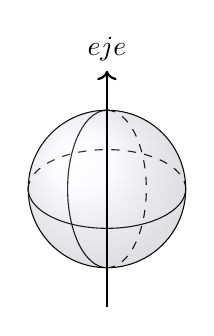
\begin{tikzpicture}
	\draw (-1,0) arc (180:360:1cm and 0.5cm);
	\draw[dashed] (-1,0) arc (180:0:1cm and 0.5cm);
	\draw (0,1) arc (90:270:0.5cm and 1cm);
	\draw[dashed] (0,1) arc (90:-90:0.5cm and 1cm);
	\draw (0,0) circle (1cm);
	\shade[ball color=blue!10!white,opacity=0.20] (0,0) circle (1cm);
	\draw[thick,->] (0,-1.5,0) -- (0,1.5,0) node[above]{$eje$};
	\end{tikzpicture}
\tab
	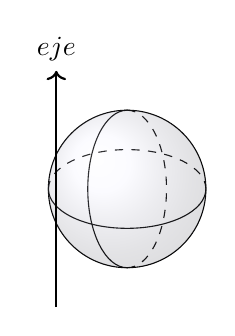
\begin{tikzpicture}
	\draw (-1,0) arc (180:360:1cm and 0.5cm);
	\draw[dashed] (-1,0) arc (180:0:1cm and 0.5cm);
	\draw (0,1) arc (90:270:0.5cm and 1cm);
	\draw[dashed] (0,1) arc (90:-90:0.5cm and 1cm);
	\draw (0,0) circle (1cm);
	\shade[ball color=blue!10!white,opacity=0.20] (0,0) circle (1cm);
	\draw[thick,->] (-0.9,-1.5,0) -- (-0.9,1.5,0) node[above]{$eje$};
	\end{tikzpicture}
	$$
Por ejemplo, en la figura, suponiendo que es una esfera que pesa toneladas, la intuición nos dice sin hacer cálculos que costará menos rotar la esfera respecto al primer eje que rotarla  respecto al segundo (y estamos en lo cierto).
\end{example}
%% Apéndices (ejercicios, exámenes)
\appendix


\chapter{Ejercicios}
% -*- root: ../GeoTopo17.tex -*-
\section{Hoja 1}
\begin{problem}[1]Responde brevemente a las siguientes preguntas:
	\ppart Si $T=T(\overline{x},\overline{y})$ y $S=S(\overline{x},\overline{y})$ son tensores, ¿lo es $T(\overline{x},\overline{y})\cdot S(\overline{x},\overline{y})$?¿y $T(\overline{x},\overline{y})+S(\overline{x},\overline{y})$?
	\ppart ¿Es $T(\overline{x},\overline{y})=\overline{x}+\overline{y}$ una aplicación bilineal?
	\ppart ¿Cuántas componentes tiene un tensor (r,s) con $V=ℝ^{m}$?
	\ppart ¿Es un tensor la aplicación que dados dos vectores de $ℝ^{3}$ les asigna la primera coordenada de su producto vectorial?
	\ppart ¿Es un tensor la aplicación que a cada par de vectores de $ℝ^{2}$ con la base canónica les asigna el área del paralelogramo que determinan?
	
	\solution
	\doneby{Jose}\\
	\spart Tenemos $$\appl{T}{ℝ^{n}×ℝ^{n}}{ℝ};\tab\appl{S}{ℝ^{n}×ℝ^{n}}{ℝ};\tab\text{ambos multilineales}$$\indent Es fácil observar que $T\cdot S(\overline{x},\overline{y})=T(\overline{x},\overline{y})\cdot S(\overline{x},\overline{y})$ no es multilineal , ya que $$T\cdot S(\alpha\cdot\overline{x},\overline{y})=\alpha^2\cdot T\cdot S(\overline{x},\overline{y})$$ \indent luego no es tensor.\newline
	\indent Si ahora nos fijamos en $T+S(\overline{x},\overline{y})=T(\overline{x},\overline{y})+S(\overline{x},\overline{y})$ es inmediato comprobar que es \indent un tensor 2 veces covariante:
	$$T+S(\alpha\cdot\overline{x},\overline{y})=T(\alpha\overline{x},\overline{y})+S(\alpha\overline{x},\overline{y})=\alpha\cdot(T+S(\overline{x},\overline{y}))$$
	$$T+S(\overline{x}_1+\overline{x}_2,\overline{y})=T(\overline{x}_1,\overline{y})+S(\overline{x}_1,\overline{y})+T(\overline{x}_2,\overline{y})+S(\overline{x}_2,\overline{y})=(T+S(\overline{x}_1,\overline{y}))+(T+S(\overline{x}_2,\overline{y}))$$
	\spart \indent Inmediato comprobar que no es bilineal multiplicando una variable por un escalar: $$T(\alpha\overline{x},\overline{y})=\alpha\overline{x}+\overline{y}\neq\alpha(\overline{x}+\overline{y})$$
	\newpage
	\spart $$\appl{T}{\underbrace{(ℝ^{m})^{*}×\cdots×(ℝ^{m})^{*}}_{\text{r veces}}×\underbrace{ℝ^{m}×\cdots×ℝ^{m}}_{\text{s veces}}}{ℝ}$$ \indent luego habrá $m^{r+s}$ componentes.
	
	\spart  Hay dos formas, una es considerar:
	\begin{align*}
		\appl{T}{ℝ^{3}×ℝ^{3}&}{ℝ} \\
		T\left(\begin{pmatrix}x_1\\x_2\\x_3\end{pmatrix},\begin{pmatrix}y_1\\y_2\\y_3\end{pmatrix}\right) &\longmapsto{x_2\cdot y_3-x_3\cdot y_2}
	\end{align*}
 	y comprobar que efectivamente se cumplen las condiciones de multilinealidad. \\
 	La segunda es considerar:
 	\begin{align*}
 		\appl{T}{ℝ^{3}×ℝ^{3}&}{ℝ} \\
 		T\left(\begin{pmatrix}x_1\\x_2\\x_3\end{pmatrix},\begin{pmatrix}y_1\\y_2\\y_3\end{pmatrix}\right) &\longmapsto{(\overline{x}×\overline{y})\cdot\overline{e}_1=\begin{vmatrix}
 				1 & 0 &  0 \\ 
 				x_1 & x_2 & x_3 \\ 
 				y_1 & y_2 & y_3 \\ 
 		\end{vmatrix}}
 	\end{align*}
	y como vimos que el determinante es multilineal, pues ya está demostrado porque es un determinante.
	
	\spart 
		\begin{align*}
		\appl{T}{ℝ^{2}×ℝ^{2}&}{ℝ} \\
		T(\overline{x},\overline{y}) &\longmapsto{A=\text{área}}
	\end{align*}
\indent El área siempre es $\geq 0$, luego si multiplico por $\lambda=-1$ tenemos $T(\lambda\overline{x},\overline{y})\neq\lambda T(\overline{x},\overline{y})$
	
\end{problem}

\begin{problem}[3] Halla cuántas componentes nulas y cuántas componentes no nulas tiene el tensor determinante en $ℝ^{n}$. Estudia cuántas son positivas.
	
	\solution
	
\end{problem}	


\bibliography{../Apuntes}{}
\printindex
\end{document}
